\documentclass[13pt]{beamer}
%
% Choose how your presentation looks.
%
% For more themes, color themes and font themes, see:
% http://deic.uab.es/~iblanes/beamer_gallery/index_by_theme.html
%
\mode<presentation>
{
\usetheme{CambridgeUS}     % or try Darmstadt, Madrid, Warsaw, ...
\usecolortheme{beaver} % or try albatross, beaver, crane, ...
\usefonttheme{default}  % or try serif, structurebold, ...
\setbeamertemplate{navigation symbols}{}
\setbeamertemplate{caption}[numbered]
} 

\usepackage[english]{babel}
\usepackage[utf8x]{inputenc}
\usepackage{xcolor}
\usepackage{multicol}
\usepackage{tikz}
\usepackage{tikz-uml}
\tikzumlset{font=\footnotesize\ttfamily}
\usepackage{hyperref}

\usepackage{listings}
\definecolor{codegreen}{rgb}{0,0.6,0}
\definecolor{codegray}{rgb}{0.5,0.5,0.5}
\definecolor{codepurple}{rgb}{0.58,0,0.82}
\definecolor{backcolour}{rgb}{0.95,0.95,0.92}

\lstdefinestyle{myCustomCppStyle}{
language=C++,
numbers=left,
stepnumber=1,
numbersep=9pt,
tabsize=2,
showspaces=false,
showstringspaces=false
}

\lstset{basicstyle=\tiny,style=myCustomCppStyle}

\lstdefinestyle{mystyle}{
backgroundcolor=\color{backcolour},   
commentstyle=\color{codegreen},
keywordstyle=\color{magenta},
numberstyle=\tiny\color{codegray},
stringstyle=\color{codepurple},
basicstyle=\ttfamily\footnotesize,
breakatwhitespace=false,         
breaklines=true,                 
captionpos=b,                    
keepspaces=true,                 
numbers=left,                    
numbersep=5pt,                  
showspaces=false,                
showstringspaces=false,
showtabs=false,                  
tabsize=1
}

\lstset{style=mystyle}

\usepackage{graphicx}
\graphicspath{ {./images/} }

\usepackage{tikz}
\usetikzlibrary{decorations.text}
\usetikzlibrary{shapes.geometric, arrows, positioning, calc, matrix}

\tikzset{
basic box/.style={
shape=rectangle, rounded corners, align=center,
draw=#1, fill=#1!25},
header node/.style={
Minimum Width=header nodes,
font=\strut\Large\ttfamily,
text depth=+0pt,
fill=white, draw},
header/.style={%
inner ysep=+1.5em,
append after command={
\pgfextra{\let\TikZlastnode\tikzlastnode}
node [header node] (header-\TikZlastnode) at (\TikZlastnode.north) {#1}
node [span=(\TikZlastnode)(header-\TikZlastnode)] at (fit bounding box) (h-\TikZlastnode) {}
}
},
hv/.style={to path={-|(\tikztotarget)\tikztonodes}},
vh/.style={to path={|-(\tikztotarget)\tikztonodes}},
fat blue line/.style={ultra thick, blue}
}

\definecolor{mygray}{RGB}{208,208,208}
\definecolor{mymagenta}{RGB}{226,0,116}
\newcommand*{\mytextstyle}{\sffamily\Large\bfseries\color{black!85}}
\newcommand{\arcarrow}[3]{%
% inner radius, middle radius, outer radius, start angle,
% end angle, tip protusion angle, options, text
\pgfmathsetmacro{\rin}{1.7}
\pgfmathsetmacro{\rmid}{2.2}
\pgfmathsetmacro{\rout}{2.7}
\pgfmathsetmacro{\astart}{#1}
\pgfmathsetmacro{\aend}{#2}
\pgfmathsetmacro{\atip}{5}
\fill[mygray, very thick] (\astart+\atip:\rin)
                 arc (\astart+\atip:\aend:\rin)
-- (\aend-\atip:\rmid)
-- (\aend:\rout)   arc (\aend:\astart+\atip:\rout)
-- (\astart:\rmid) -- cycle;
\path[
decoration = {
 text along path,
 text = {|\mytextstyle|#3},
 text align = {align = center},
 raise = -1.0ex
},
decorate
](\astart+\atip:\rmid) arc (\astart+\atip:\aend+\atip:\rmid);
}
\title[Design Pattern]{Behavioral Design Pattern}
\author{Hung Tran}
\institute{Fpt software}
\date{\today}


\begin{document}

\begin{frame}
\titlepage
\end{frame}

% Uncomment these lines for an automatically generated outline.
\begin{frame}{Outline}
\tableofcontents
\end{frame}

\section{Behavioral Pattern Overview}

\begin{frame}{Behavioral Pattern Overview}
	\begin{center}
	\textcolor{blue}{\textbf{Behavioral design patterns are concerned with algorithms and the assignment of responsibilities between objects.}}
	\end{center}
	\begin{itemize}
		\item \textbf{Chain of responsibility}: lets you pass requests along a chain of handlers.
		\item \textbf{Command}: turns a request into a stand-alone object that contains all information about the request.
		\item \textbf{Iterator}: lets you traverse elements of a collection without exposing its underlying representation (list, stack, tree, etc.).
		\item \textbf{Mediator}: lets you reduce chaotic dependencies between objects.
		\item \textbf{Memento}: lets you save and restore the previous state of an object without revealing the details of its implementation.
	\end{itemize}
\end{frame}

\begin{frame}{Behavioral Pattern Overview}
	\begin{itemize}
		\item \textbf{Observer}: lets you define a subscription mechanism to notify multiple objects about any events that happen to the object they’re observing.
		\item \textbf{State}: lets an object alter its behavior when its internal state changes. It appears as if the object changed its class.
		\item \textbf{Strategy}: lets you define a family of algorithms, put each of them into a separate class, and make their objects interchangeable.
		\item \textbf{Template Method}: defines the skeleton of an algorithm in the superclass but lets subclasses override specific steps of the algorithm without changing its structure.
		\item \textbf{Visitor}: lets you separate algorithms from the objects on which they operate.
	\end{itemize}
\end{frame}

\section{Command pattern}

\begin{frame}{Problem Statement: text-editor app}
	\begin{columns}[T]
		\begin{column}{.5\textwidth}
			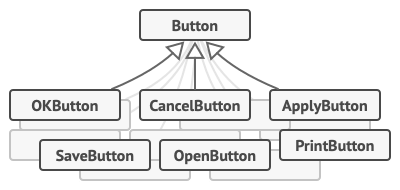
\includegraphics[scale=0.4]{./images/problem.png}
			\begin{itemize}
				\item Create a toolbar with a bunch of buttons for various operations of the editor.
				\item Created a very neat Button class that can be used for buttons on the toolbar, as well as for generic buttons in various dialogs.
			\end{itemize}
		\end{column}
	
		\begin{column}{.5\textwidth}
			\begin{itemize}
				\item While all of these buttons look similar, they’re all supposed to do different things.
				\item Where would you put the code for the various click handlers of these buttons? 
				\item The simplest solution is to create tons of subclasses for each place where the button is used.
			\end{itemize}
			\textcolor{red}{You have an enormous number of subclasses and multiple ways to do the same operation.}
		\end{column}
	\end{columns}
\end{frame}

\begin{frame}{The principle of separation of concerns}
	\begin{center}
		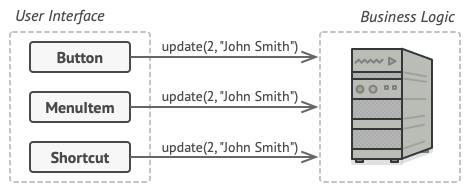
\includegraphics[scale=0.5]{./images/solution1.png}
	\end{center}
	\begin{itemize}
		\item A layer for the graphical user interface.
		\item Another layer for the business logic.
		\item The GUI layer is responsible for rendering a beautiful picture on the screen, capturing any input and showing results of what the user and the app are doing.
	\end{itemize}
\end{frame}

\begin{frame}{The command pattern}
	\begin{center}
		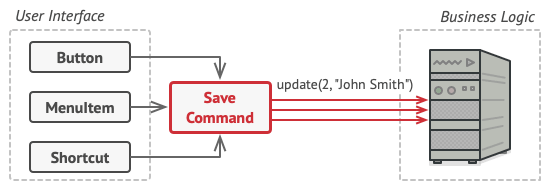
\includegraphics[scale=0.5]{./images/solution.png}
	\end{center}
	\begin{itemize}
		\item The Command pattern suggests that GUI objects shouldn’t send these requests directly.
		\item You should extract all of the request details, such as the object being called, the name of the method and the list of arguments.
		\item Command objects serve as links between various GUI and business logic objects.
		\item The GUI object doesn’t need to know what business logic object will receive the request and how it’ll be processed.
	\end{itemize}
\end{frame}

\begin{frame}{The Intent of Command Design Pattern}
	\begin{center}
	\textcolor{red}{\textbf{Command is a behavioral design pattern that turns a request into a stand-alone object that contains all information about the request. This transformation lets you pass requests as a method arguments, delay or queue a request’s execution, and support undoable operations.}}\\
	\end{center}
\end{frame}

\begin{frame}{Structure of Command Pattern}
	\begin{center}
	\begin{tikzpicture}
 	\umlemptyclass[x=0,y=0]{Client}
 	\umlclass[x=5,y=0]{Handler}{-nextHandler}{+handlerRequest() \\ +setNextHandler()}
 	\umlclass[x=3,y=-4]{ConcreteHandle1}{}{+handlerRequest()}
 	\umlclass[x=7,y=-4]{ConcreteHandle2}{}{+handlerRequest()}
 	\umluniassoc[pos=0.95, align=right, name=uniassoc]{Client}{Handler}
 	\umlinherit[geometry=|-|, pos=0.95, align=right, name=uniassoc]{ConcreteHandle1}{Handler}
 	\umlinherit[geometry=|-|, pos=0.95, align=right, name=uniassoc]{ConcreteHandle2}{Handler}
	\end{tikzpicture}	
	\end{center}
\end{frame}

\begin{frame}{Basic implementation: bulb class}
\begin{columns}[T]
\begin{column}{.45\textwidth}
\lstset{basicstyle=\tiny,style=myCustomCppStyle}
bulb.h
\lstinputlisting{./examples/bulb/bulb.h}
\end{column}

\begin{column}{.45\textwidth}
\lstset{basicstyle=\tiny,style=myCustomCppStyle}
bulb.cpp
\lstinputlisting{./examples/bulb/bulb.cpp}

command.h
\lstinputlisting{./examples/bulb/command.h}
\end{column}
\end{columns}
\end{frame}

\begin{frame}{Basic implementation: TunOn class}
\begin{columns}[T]
\begin{column}{.45\textwidth}
\lstset{basicstyle=\tiny,style=myCustomCppStyle}
turnOn.h
\lstinputlisting{./examples/bulb/turnOn.h}
\end{column}

\begin{column}{.45\textwidth}
\lstset{basicstyle=\tiny,style=myCustomCppStyle}
turnOn.cpp
\lstinputlisting{./examples/bulb/turnOn.cpp}
\end{column}
\end{columns}
\end{frame}

\begin{frame}{Basic implementation: TurnOff class}
\begin{columns}[T]
\begin{column}{.45\textwidth}
\lstset{basicstyle=\tiny,style=myCustomCppStyle}
turnOff.h
\lstinputlisting{./examples/bulb/turnOff.h}
\end{column}

\begin{column}{.45\textwidth}
\lstset{basicstyle=\tiny,style=myCustomCppStyle}
turnOff.cpp
\lstinputlisting{./examples/bulb/turnOff.cpp}
\end{column}
\end{columns}
\end{frame}

\begin{frame}{Basic implementation: remote class}
\begin{columns}[T]
\begin{column}{.45\textwidth}
\lstset{basicstyle=\tiny,style=myCustomCppStyle}
remote.h
\lstinputlisting{./examples/bulb/remote.h}
\end{column}

\begin{column}{.45\textwidth}
\lstset{basicstyle=\tiny,style=myCustomCppStyle}
remote.cpp
\lstinputlisting{./examples/bulb/remote.cpp}
\end{column}
\end{columns}
\end{frame}

\begin{frame}{Basic implementation: main}
\begin{columns}[T]
\begin{column}{.45\textwidth}

\end{column}

\begin{column}{.45\textwidth}
\lstset{basicstyle=\tiny,style=myCustomCppStyle}
main.cpp
\lstinputlisting{./examples/bulb/main.cpp}
\end{column}
\end{columns}
\end{frame}

\begin{frame}{Applicability}
	\begin{itemize}
		\item Use the Command pattern when you want to parametrize objects with operations.
		\item Use the Command pattern when you want to queue operations, schedule their execution, or execute them remotely.
		\item Use the Command pattern when you want to implement reversible operations..
	\end{itemize}
\end{frame}

\begin{frame}{How to Implement}
	\begin{itemize}
		\item Declare the command interface with a single execution method.
		\item Start extracting requests into concrete command classes that implement the command interface. Each class must have a set of fields for storing the request arguments along with a reference to the actual receiver object. All these values must be initialized via the command’s constructor.
		\item Identify classes that will act as senders. Add the fields for storing commands into these classes. Senders should communicate with their commands only via the command interface. Senders usually don’t create command objects on their own, but rather get them from the client code.
		\item Change the senders so they execute the command instead of sending a request to the receiver directly.
		\item The client should initialize objects in the following order:
		    Create receivers.
		    Create commands, and associate them with receivers if needed.
		    Create senders, and associate them with specific commands.
	\end{itemize}
\end{frame}

\begin{frame}{Pros and Cons}
	\begin{columns}[T]
		\begin{column}{.5\textwidth}
			\begin{itemize}
				\item Single Responsibility Principle. You can decouple classes that invoke operations from classes that perform these operations.
				\item Open/Closed Principle. You can introduce new commands into the app without breaking existing client code.
				\item You can implement undo/redo.
				\item You can implement deferred execution of operations.
				\item You can assemble a set of simple commands into a complex one.
			\end{itemize}
		\end{column}
	
		\begin{column}{.5\textwidth}
			\begin{itemize}
				\item The code may become more complicated since you’re introducing a whole new layer between senders and receivers.
			\end{itemize}
		\end{column}
	\end{columns}
\end{frame}

\begin{frame}{Relations with Other Patterns}
	\begin{itemize}
		\item Chain of Responsibility, Command, Mediator and Observer address various ways of connecting senders and receivers of requests:
		\item Handlers in Chain of Responsibility can be implemented as Commands. In this case, you can execute a lot of different operations over the same context object, represented by a request.
		\item You can use Command and Memento together when implementing “undo”. In this case, commands are responsible for performing various operations over a target object, while mementos save the state of that object just before a command gets executed.
		\item Command and Strategy may look similar because you can use both to parameterize an object with some action. However, they have very different intents.
		\item Prototype can help when you need to save copies of Commands into history.
		\item You can treat Visitor as a powerful version of the Command pattern. Its objects can execute operations over various objects of different classes.
	\end{itemize}
\end{frame}

\begin{frame}
\begin{center}
{\fontsize{40}{50}\selectfont Thank You!}
\end{center}
\end{frame}

\end{document}
